\section{Partie 3: Etude de performance et optimisations}
%\paragraph{}Je me suis finalement penché sur les performances de la version 3D de NTMIX développé au cours de ce stage. J'ai dans un premier temps étudié les performances séquentielles du programme (code tel qu'il était à la fin de la première partie) puis les performances de la version parallèle.
\subsection{Présentation du matériel}
L'ensemble des tests suivants ont été réalisés sur les calculateurs internes du CERFACS, le Bullx B510 (neptune) et le cluster LENOVO (nemo). Ils possèdent les caractéristiques suivantes:

\begin{table}[h]
  \begin{center}
    \begin{tabular}{|M{3.5cm}|M{5cm}|M{5cm}|}
      \hline
      & Bullx & Lenovo \\
      \hline
      Noeuds & 158 & 252 \\
      \hline
      Puissance crête & 53 TFlop/s & 242 TFlop/s \\
      \hline
      Consommation maximale applicative & 51 kW.h & 73 kW.h \\
      \hline
      Consommation à vide & 25 kW.h & 34 kW.h \\
      \hline
      Processeurs & Intel Sandy Bridge bi-socket, 8 coeurs (2.6 GHz) & Intel Haswell bi-socket, 12 coeurs (2.5 GHz) \\
      \hline
      Mémoire & 32 Go de mémoire cadencée à 1.6 GHz & 64 Go de mémoire cadencée à 2.133 GHz \\
      \hline
    \end{tabular}
  \end{center}
  \caption{\label{tab:carac}Caractéristiques des calculateurs du Cerfacs}
\end{table}

%\begin{figure}[ht]
%  \centering
%  \begin{minipage}{.5\textwidth}
%    \centering
%    \includegraphics[width=.7\linewidth]{figures/neptune.jpg}
%    \caption{\label{fig:neptune}Neptune}
%  \end{minipage}%
%  \begin{minipage}{.5\textwidth}
%    \centering
%    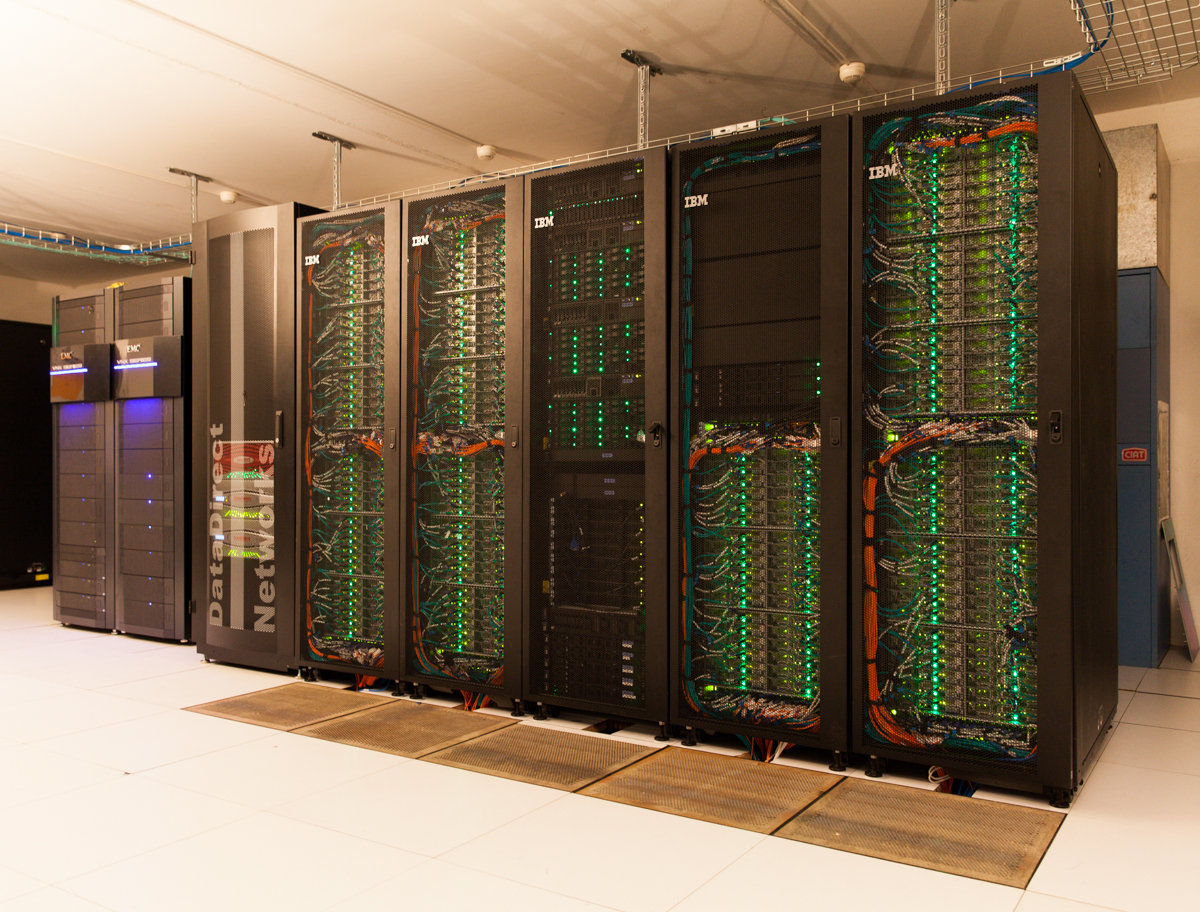
\includegraphics[width=.9\linewidth]{figures/nemo.jpg}
%    \caption{\label{fig:neptune_node}Nemo}
%  \end{minipage}
%\end{figure}

\subsection{Métriques utilisées}
Le temps d'exécution pour calculer un point pour un pas de temps ($\mu s/it/p$). Plus cette valeur est basse, plus le code est efficace. 

\subsection{Performances séquentielles}
Dans cette partie, on s'interresse au programme testé et fonctionnel présenté dans la première partie. Avant de commmencer à profiler l'application, 3 cas ont été définis; ils permettent de couvrir une plus grande partie du code; en effet chacun de ces cas utilise des parties du code différentes:
\begin{itemize}
\item Cas périodique: le domaine de calcul est périodique
\item Cas non-périodique: dans ce cas, les frontières sont traitées
\item Cas symétrique: des méthodes de dérivations différentes sont utilisées
\end{itemize}

On part d'une taille de 20 points de coté (donc la taille du domaine est de $20\times20\times20$ points) et on l'augmente par pas de 50\%. Pour chacune de ces tailles de domaine, on réalise 20 itérations et on calcule la moyenne des temps par points de celles-ci.

%Une fois le programme testé et fonctionnel, j'ai commencé à étudier ses performances. J'ai, dans un premier temps, mesuré un temps de référence pour l'exécution de ce programme; compilation par défaut, donc avec l'option -O2.

\subsubsection{Vectorisation}
L'application est constituée de nombreuses boucles de calculs parcourant les tableaux contenant les variables conservatives. Il semble donc être un bon candidat pour la vectorisation. La vectorisation est présente sur les processeurs possédant des instructions SIMD (Single Instruction Multiple Data). On peut donc appliquer une opération sur plusieurs éléments à la fois au lieu d'un seul. Comme on peut le voir sur la figure \ref{fig:simd}, si on à une boucle calculant la somme de 2 tableaux, sans vectorisation, le processeurs réalisera une addition à la fois mais avec, il peut traiter plus d'éléments à la fois.


Sur LENOVO, le jeu d'instruction AVX2 est disponible, il permet de traiter des vecteurs de 256 octets, soit 4 nombre double précision. Si les boucles réalise beaucoup de calculs, on peut donc esperer diviser le temps par 4. Cependant, comme on peut le constater sur la figure \ref{fig:bench_scal_nemo}, la vectorisation n'a entraînée qu'un gain d'entre 18 et 25\% selon le cas. Grâce à Intel Advisor, qui permet d'analyser les boucles qui ont été vectorisées, il est possible de voir que:
\begin{itemize}
\item Certaines fonctions dans lesquelles le programme passe beaucoup de temps ne sont pas vectorisée à cause de dépendances, nottamment dans le calculs des gradients. Dans ce cas, on est dépendant de la méthode utilisée pour ces calculs et on ne peut pas forcer la vectorisation de ces boucles.
\item Beaucoup de petites boucles de calcul ne sont pas vectorisées. Ceci est dû à la structure de la mémoire du programme; tous les tableaux contennant des variables conservatives sont en réalité des sous-parties d'un plus grand tableaux. Lorsque des opérations sont effectuées sur ces tableaux, le compilateur assume qu'elle travaille sur un unique grand tableau et empêche donc la vectorisation au profit de la cohérence. Pour résoudre ce problème, il suffit d'indiquer au compilateur qu'il n'y a pas aliasing; on garantit ainsi qu'une zone mémoire ne peut être accédée que par un nom et que le programme ne dépassera pas les limites d'un tableau.
\end{itemize}



(memory bound)



\begin{figure}[h!]
  \centering
  \begin{subfigure}[b]{0.5\textwidth}
    \centering
    \includegraphics[page=1,scale=0.6]{gnuplot/bench_scalaire_nemo.pdf}
  \caption{\label{fig:bench_scal_nemo_nonper}}
  \end{subfigure}%
  ~
  \begin{subfigure}[b]{0.5\textwidth}
    \centering
    \includegraphics[page=2,scale=0.6]{gnuplot/bench_scalaire_nemo.pdf}
  \caption{\label{fig:bench_scal_nemo_sym}}
  \end{subfigure}
  \begin{subfigure}[b]{0.5\textwidth}
    \centering
    %\includepdf[pages={2}]{gnuplot/bench_scalaire.pdf}
    \includegraphics[page=3,scale=0.6]{gnuplot/bench_scalaire_nemo.pdf}
  \caption{\label{fig:bench_scal_nemo_per}}
  \end{subfigure}
  \caption{\label{fig:bench_scal_nemo}Temps par points des cas tests - LENOVO}
\end{figure}


\begin{figure}[h!]
  \centering
  \begin{subfigure}[b]{0.5\textwidth}
    \centering
    \includegraphics[page=1,scale=0.6]{gnuplot/bench_scalaire_neptune.pdf}
  \caption{\label{fig:bench_scal_neptune_nonper}}
  \end{subfigure}%
  ~
  \begin{subfigure}[b]{0.5\textwidth}
    \centering
    \includegraphics[page=2,scale=0.6]{gnuplot/bench_scalaire_neptune.pdf}
  \caption{\label{fig:bench_scal_neptune_sym}}
  \end{subfigure}
  \begin{subfigure}[b]{0.5\textwidth}
    \centering
    %\includepdf[pages={2}]{gnuplot/bench_scalaire.pdf}
    \includegraphics[page=3,scale=0.6]{gnuplot/bench_scalaire_neptune.pdf}
  \caption{\label{fig:bench_scal_neptune_per}}
  \end{subfigure}
  \caption{\label{fig:bench_scal_neptune}Temps par points des cas tests - BULL}
\end{figure}




\subsubsection{Alignement de la mémoire}
blabla marche pas

%\paragraph{durée=f(taille)}


\subsection{Performances parallèle}


%\subsubsection{Méthode de communication}
%Avant de comparer les méthodes de recouvrement, je me suis dans un premier temps interréssé aux méthodes de communication utilisées pour la première méthode (\ref{sec:}). Pour cela, j'ai comparer la durée passée dans des communications pour chacune des méthode et ceux pour différentes taille de grille.


%mesurer le temps d'exécution par point par pas de temps de chacune des méthodes pour différentes taille de grille.


%\subsubsection{Méthode de recouvrement}
%Je compare ici les 2 méthodes utilisée pour le recouvrement de domain présentées dans la partie précedente. Pour rappel: 





%\subsubsection{Décomposition du domaine}
%Le découpage du domaine est entièrement configurable par l'utilisateur, nous verons donc ici l'influence que ce découpage peut avoir sur le temps d'exécution du programme. 

%https://www.sharcnet.ca/help/index.php/Measuring_Parallel_Scaling_Performance
\subsection{Scalabilité}

\subsubsection{Scalabilité forte}
Pour une taille de problème fixée, on augmente le nombre de processus. Dans le cas d'une application réalisant beaucoup de calculs, le but est de trouver le le point auquel on obtient un temps d'exécution raisonnable mais en limitant les surcoût induit par un programme paralléle. 	

\subsubsection{Scalabilité faible}
Dans ce cas, la taille du problème assignée à chaque processus reste constante et on ajoute des processeurs dans le but d'augenter la taille globale du problème. Etant donné que le pattern de communication ne change pas (chaque processus communique avec ses voisins directs), le but est de mettre en évidence le coût des communications globales (ici les reduce pour le calcul du pas de temps maximal).


